\documentclass{article}
\usepackage[utf8]{inputenc}

\usepackage{amsmath}
\usepackage{amssymb}
\usepackage{graphicx}
\usepackage{tikz}
\usepackage{geometry}
 \geometry{
 a4paper,
 total={210mm,297mm},
 left=10mm,
 top=30mm,
 right=10mm
 }

\graphicspath{{./}}
\newcommand*\circled[1]{\tikz[baseline=(char.base)]{
    \node[shape=circle,draw,inner sep=0.5pt] (char) {#1};}}

\title{
\normalfont \large 
\textsc{Indian Institute of Technology, Ropar} \\    [40pt] 
\horrule{} \\[0.4cm] 
\Huge CS204 Course Project - Phase III\\ 
\horrule{} \\[0.5cm]
\protect\vspace{2.0cm}
\large
\textup{Team Members:}\\\vspace{1cm}
\begin{centering}
\begin{enumerate}
    \item Aditya Agarwal - 2019CSB1064
    \item Aneeket Mangal - 2019CSB1071
    \item Fadia Het Rakeshkumar - 2019CSB1084
    \item Shikhar Soni - 2019CSB1119
    \item Tanmay Aeron - 2019CSB1124
\end{enumerate}
\end{centering}
\date{}
\centering
\protect\vspace{4.0cm}

\includegraphics[width=1.0\textwidth]{riscv-logo-1.png}
}

\pagenumbering{roman}
\begin{document}
\maketitle
\newpage
\begin{centering}
\begin{Huge}
\textsf{Project Description}\\
\end{Huge}
\end{centering}
\protect\vspace{2.0cm}
\LARGE
The aim of this project is to simulate the machine level execution of RISC V as well as the execution of RISC-V 32-bit instructions using a high level language.\\

The Project also aims to give updates to the user regarding each step of the execution of the program. It also returns the final status of the memory and registers as output for the user to analyse the working of their programs thoroughly.\\

The project can also be executed using step functionality for debugging purposes.\\

The Project currently allows the user to use 29 different instructions and can be extended to allow the use of any number of instructions by editing the .csv files as long as the instructions are supported by 32-bit RISC V ISA. \\

The Project also allows the user to choose which replacement policy to be used and which branch prediction to used while executing the instructions of the instructions.\\

The program supports a configurable design that will allow the user to select whether or not they want pipelining, data forwarding, user defined cache sizes, etc. to analyse the working and performance of different codes and their behaviour under different hardware conditions.\\

The program executes each instruction using five stages as described in the RISC V architecture and gives out all sort of stats and the opportunity to observe the behaviour and output of the program for each cycle as per the user's convenience.\\
\newpage
The several options given to the user regarding the configuration of the virtual hardware that runs the machine codes are as follows.\\
\begin{enumerate}
  \item {\bf Pipeling:} If ticked allows pipelined execution of instructions.
  \item {\bf Forwarding:} If ticked allows forwarding to resolve data hazards otherwise the program uses stalling to do the same.
  \item {\bf Machine Code:} If ticked allows the user to directly provide machine code through the editor, expects assembly code otherwise.
  \item {\bf I\$ and D\$:} I\$ refers to the instruction cache (from where the instructions are fetched during fetch stage) and D\$ refers to the data cache (where all sorts of data needed by the program is stored and read from).
  \item{\bf Cache:} Allows the user to specify the total cache size for each of the two caches.
  \item {\bf Block:} Allows the user to specify the total block size for each of the two caches.
  \item{\bf Ways:} Allows the user to choose an N-way set associative cache for each of the cache. 'N' being the number entered in this column by the user.
  \item{\bf Replacement:} Refers to the block replacement policy you want each of your caches to follow.
  \item{\bf Branch Predictor:} Allows you to select the among different branch prediction methods such as Always Taken (AT), Always Not Taken (ANT), Backward Taken Forward Not Taken (BTFNT), One Bit dynamic branch predictor (1-Bit) and Two Bit dynamic branch predictor (2-Bit).
  \item{\bf Initial State:} Allows the user to decide the initial state for all the dynamic branch predictors.
\end{enumerate}\\

\newpage
\begin{centering}
\begin{Huge}
\begin{bf}
\vspace{2.0cm}
\textsf{Technologies employed}\\
\end{bf}
\end{Huge}
\end{centering}
\protect\vspace{2.0cm}
\textbf{}
\huge
Back-end - Python3
\begin{enumerate}
  \item {\bf pandas} for reading {\bf .csv} files.
  \item {\bf os} for getting and adding path to certain file locations.
  \item {\bf collections.defaultdict} to make a hash map for memory.
  \item {\bf sys} for reading and editing files with ease.
  \item {\bf json} for crunching data
  \item {\bf glob} for file management
  \item {\bf regex} for making the cleaned file
  \item {\bf random} for generating random number in Random Replacement Policy
  \item {\bf argparse} for taking arguments from the user
\end{enumerate}\\
\textbf{}

Front-end - Python3
\begin{enumerate}
  \item {\bf PyQt5} for the Graphic User Interface.
  \item {\bf qdarkstyle} for dark theme in the GUI.
  \item {\bf QtAwesome} for using icons
\end{enumerate}
\newpage
\textsl{\textbf{How to run the code:}}\\\\
\textsf{Instructions to run GUI version:}\\
\textsl{python main.py -g}\\
After running this command in the terminal, the GUI will pop up.\\
You can then enable each knob by ticking the checkbox for each.\\
For the fifth knob you can add the instruction number by adding the instruction in the box.\\
Information about the Fetch, Decode, etc. can be seen in the info tab on the right side when you click on the respective buttons in the DataPath tab
\par\noindent\rule{\textwidth}{0.4pt}
\textsf{Instructions to run Non GUI version:}\\
add `-k1' to enable knob1\\
add `-k2' to enable knob2\\
add `-k3' to enable knob3\\
add `-k4' to enable knob4\\
add `-k5 instruction number' to enable for that particular instruction\\
add `-ICache cachesize blocksize ways' for setting instruction cache details\\
add `-DCache cachesize blocksize ways' for setting data cache \\details\\
If you want to run a particular file, add that file in test folder and add `-f filename', otherwise main.mc is run\\
For example, if you want to enable knob1, knob2 , knob3, knob4 and knob5 with instruction 3, and make a data cache of size 512, block size 8 and ways to be equal to 2, and run fib.mc, write\\
\textsl{python main.py -k1 -k2 -k3 -k4 -k5 3 -DCache 512 8 2 -f fib.mc}\\
\newpage
\noindent
\textsf{Other features:}\\
\\
Arguments: [-h] [-g] [-f F] [-k1] [-k2] [-k3] [-k4] [-k5 INS] [-ICache cacheSize blockSize noOfWays] [-DCache cacheSize blockSize noOfWays]\\\\
\textsf{Description:}\\

\begin{enumerate}

  \item {[-h, -help]}        show help message and exit
  \item {[-g, -gui]}           enable GUI
  \item {[-f F, -filename F]}  specify file which is to be run, defaults to main.mc
  \item {[-k1, -knob1]}        enable Pipelining
  \item {[-k2, -knob2]}        enable Data Forwarding
  \item {[-k3, -knob3]}        show value in registerFile at end of each cycle
  \item {[-k4, -knob4]}        show value in Pipeline Registers at end of each cycle
  \item {[-k5 INS, -knob5 INS]}  show value in Pipeline Registers at end of each cycle for particular instruction
  \item {[ICache cacheSize blockSize noOfWays]} configure input cache in format cache size, block size and number of ways in Instruction Cache.
  \item {[DCache cacheSize blockSize noOfWays]} configure data cache in format cache size, block size and number of ways in Data Cache. If not specified both of the above default to 64 bytes (cache size), 4 bytes (block size), 2 (way set associative).
  \item {[-h]} for help on running the code
\end{enumerate}
\\
\newpage
\begin{centering}
\begin{Huge}
\textsf{Implementation Details}\\
\end{Huge}
\end{centering}
\protect\vspace{1.0cm}
We have implemented the project using the following method:\\

The simulator takes the input from a \textsl{\textbf{.mc}} file that contains the machine code in the required format, the content of this file can be modified using the GUI editor by supplying an assembly code that is converted to the machine code or by directly supplying the machine code directly in the required format or by changing the main.mc file.\\
Then, it stores the \textsl{\textbf{.data}} part into the data memory and the \textsl{\textbf{.text}} part in the text part of the memory.
Once that is completed, we run the program using the following method:
\begin{enumerate}
\item Instruction Fetch: PC is incremented by 4, and the instruction is loaded from the memory and stored in the Instruction Register.
\item Instruction Decode: We are identifying the instruction using the .csv file and {\bf pandas} library and returning all the required fields. The registers RA and RB are also set during this stage.
\item Execute: The ALU executes the instruction by computing the desired output using values stored in registers in RA, RB, imm, etc. The required type of ALU instruction is determined by another .csv file. We are updating the output in the RZ register.
\item Memory Access: Memory is read and written in this stage. This stage is used only for load and store instructions. For the remaining instructions, this stage is redundant. The value of the RY register is also consequently updated.
\newpage
\item Register Write-back: Here we are storing the value of the temporary register RY in the destination register, resulting in the register files being updated. The register update is extremely fast compared to memory read and update.\\
\end{enumerate}
We have implemented data forwarding by passing the required values from the source buffer to the destination buffer without the need of stalling in most cases. This helps to reduce the number of stalls required. The types of data forwarding are:\\
\begin{enumerate}
    \item Execute to Execute
    \item Memory to Execute
    \item Memory to Memory
\end{enumerate}
\vspace{1cm}

\vspace{1cm}\\
The program detects hazards present which can cause an incorrect value to be register due to one instruction's stage being executed before another. This is fixed by either transferring data values directly with the help of data forwarding, or with the help of stalling which delays the next instruction so that the previous one is updated in time.\\

While data forwarding is enabled, there is no use of stalling\\ except for one particular case where we use it along with \\Memory-to-Execute data forwarding.\\


\newpage
\begin{centering}
\begin{Huge}
\textsf{Input/Output format details}\\
\end{Huge}
\vspace{0.6cm}
\end{centering}
\noindent
\LARGE
{\bf Input Format:}\\
{\bf The input format of the RISC-V code is}\\
.data\\
array: .word 1 2 10 9 3 8 4 7 5 6\\
.text\\
auipc x11,0x10000\\
addi x11 x11 0\\
addi x12 x0,10\\
addi x31,    x0,2\\
bubblesort: \\
addi x12,x12,-1 \\
beq x12,x0,exit \\
addi x13, x0,0 \\
loop:\\
beq x13,x12,break \\
sll x14,x13,x31 \\
add x14,x14,x11 \\
lw x15,0(x14) \\
lw x16,4(x14) \\
addi x13,x13,1 \\
blt x15,x16,loop\\
beq x15,x16,loop\\
sw x16,0(x14) \\
sw x15,4(x14\\
jal x0 loop\\
break:\\
jal x0 bubblesort\\
exit:
\newpage
{\bf The input format of the Machine code is}\\
0x0 0x00500513\\
0x4 0x008000EF\\
0x8 0x0440006F\\
\$\\
0x10000000 0x64\\\\
The input is given through GUI if the GUI is run else it is taken from the main.mc file.\\\\
The section given before the `\$' sign is the text segment of the code and all the lines after it signify the data segment of the code.\\\\
Output is generated in the `generated' folder. It contains the following things:  \\
\begin{enumerate}
    \item `registers.txt' contains the register values
    \item `memory.txt' contains the data part of the memory
    \item `stats.txt' contains the statistical details of the program
    \item `outputLog.txt' contains the buffer data of each cycle
    \item `buffer.txt' contains buffer data about the instruction given after k5 knob
    \item `CacheInfo.txt' contains information about the cache
    \item 'DataCache.txt' contains information about the data cache
    \item 'InstructionCache.txt' contains information about the instruction cache
    \item `forwarding.txt' contains information about forwarding used for front end information
    \item Buffer Snapshot and Register Snapshots folders are used for front end information
    
\end{enumerate}
\newpage
Example output for Buffer.txt\\\\
Fetch: (`00000000', `00400513', `00000004') \\
Decode: (9, `00000000', `00000000', `00000000', `00000000', 10, 0, 4, `00000004', `00000004', [[False, `NO', 0], [False, `NO', 0]]) \\
Execute: (9, `00000004', 10, `00000000', 0, 4, `00000004', `00000000') \\
MemoryAccess: (9, `00000004', 10, `00000000') \\\\
Example output for Forwarding.txt\\
{``EE1": ``F", ``EE2": ``F", ``ME1": ``F", ``ME2": ``F", ``MM": ``F"}\\
Here EE1:F means forwarding of Execute to Execute between prev instruction(1 means previous instruction) and current instruction is False\\
Similarly ME2: T means forwarding from Memory to Execute from previous to previous instruction(2 means previous to previous instruction) is True\\\\
CacheInfo.txt\\
`F' stands for Fetch, `L' stands for Load and `S' stands for Store\\
In the Cache Info in Fetch the index, Set, isMiss and Victim block is printed\\
Here the isMiss = T means isMiss is True and so we found a miss\\
Similarly if Fetch or Load or Store is -1 means the corresponding instruction is not executed.\\
\\The user can specify input configurations for the Instruction Cache and Data Cache separately. Outputs for the two will also be displayed separately.\\
Input parameters that can be set by the user include:
\begin{enumerate}
    \item Cache size
    \item Cache Block size
    \item Number of ways for Set Associative
\end{enumerate}
\\Output parameters include:
\begin{enumerate}
    \item Number of accesses
    \item Number of hits
    \item Number of misses
\end{enumerate}

\newpage
\Large
\textbf{In \textsl{stats.txt} we have printed the following:}

\begin{enumerate}
\begin{LARGE}
\item \textsf{Total number of cycles}
\item \textsf{Total number of instructions executed}
\item \textsf{CPI}
\item \textsf{Data Transfer instructions executed}
\item \textsf{ALU instructions executed}
\item \textsf{Control instructions executed}
\item \textsf{Total Stall Count}
\item \textsf{Number of Data Hazards}
\item \textsf{Total Control Hazards}
\item \textsf{Total Branch misprediction}
\item \textsf{Number of stalls due to data hazards}
\item \textsf{Number of stalls due to control hazards}
\end{LARGE}
\end{enumerate}

\par\noindent\rule{\textwidth}{0.4pt}



\noindent
\textbf{An example output for \textsl{stats.txt} is :}\\
\\
\begin{LARGE}
\textsf{Total number of Cycles in the program :14}\\
\textsf{Total number of Instructions executed :4}\\
\textsf{CPI is :3.5}\\
\textsf{Data Transfer Instructions Executed :0}\\
\textsf{ALU instructions are :4}\\
\textsf{Control instructions :0}\\
\textsf{Total Stall Count are :6}\\
\textsf{Number of Data Hazards are :3}\\
\textsf{Total Control Hazards are :0}\\
\textsf{Total Branch mispredictions are :0}\\
\textsf{Number of stalls due to data hazards are :6}\\
\textsf{Number of stalls due to control hazards are :0}\\\\
\textsf{The instruction fed was:}\\
\textsf{0x0	0x00A50513}\\
\textsf{0x4	0x00A50513}\\
\textsf{0x8	0x00A50513}\\
\textsf{0xC	0x00A50513}\\
\end{LARGE}
\vspace{0.6cm}

\noindent
\newpage

\begin{Huge}
\centering{\textsf{Graphical User Interface}}\\
\end{Huge}
\vspace{2cm}
\begin{centering}
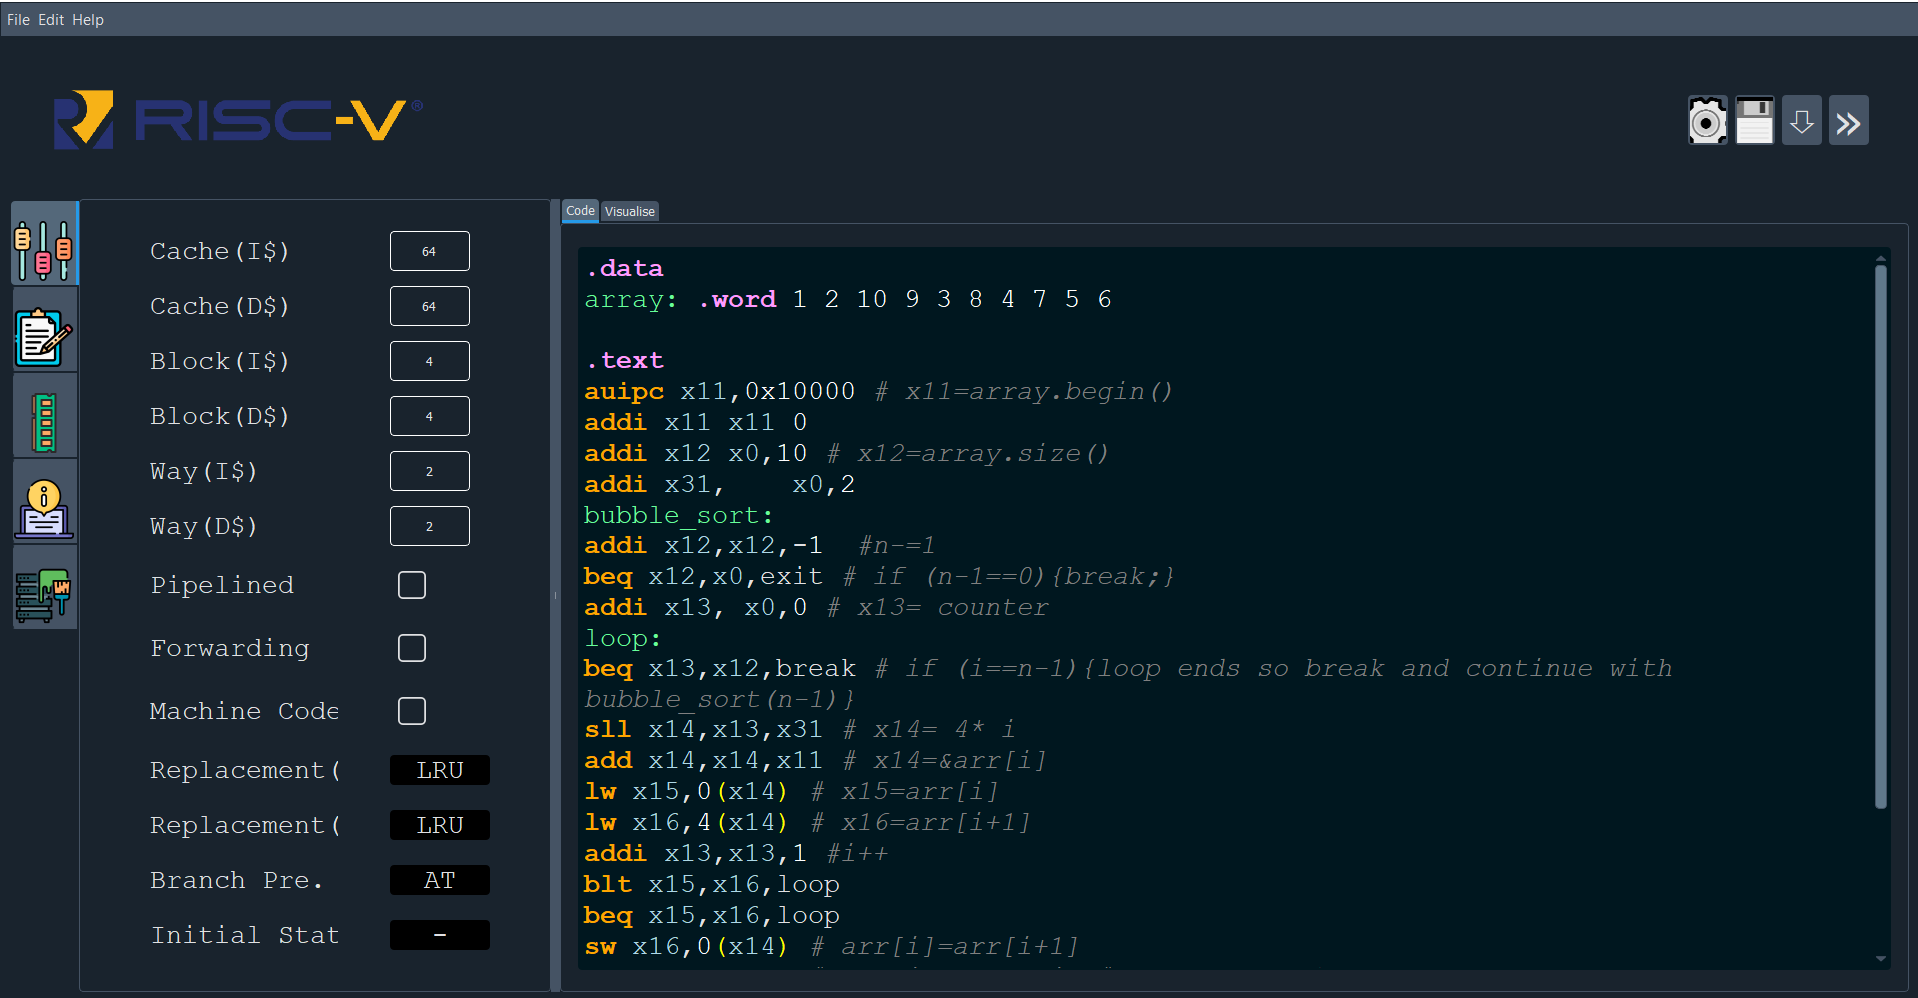
\includegraphics[width=1.0\textwidth]{FrontGUI.png}\vspace{2cm}
\end{centering}
Above is the GUI image, the tab on the right is the `controls tab' and the user can change the knobs and cache configurations accordingly (cache size must be greater than the block size and the cache size should be a power of 2  along with the block size being a multiple of 4 to ensure word alignment).\\
\unindent
We can input the Cache Size, Block Size (in bytes) and Ways on the right side of the page.\\
We can enable the knobs by ticking the corresponding boxes, for knob5 one needs to enter the instruction number on the 'k6' block (if no number is entered then it defaults to 1).
We can compile the code by pressing the `Settings/Compile' icon corresponding to compile, there's also the save icon below it represented by a `floppy disk'.\\
We can also change the theme by clicking the `bulb button' to change from light to dark mode and vice versa.
\unindent
When we press the compile button the code in the editor gets saved in main.mc and the code will be executed.
\newpage
\begin{centering}
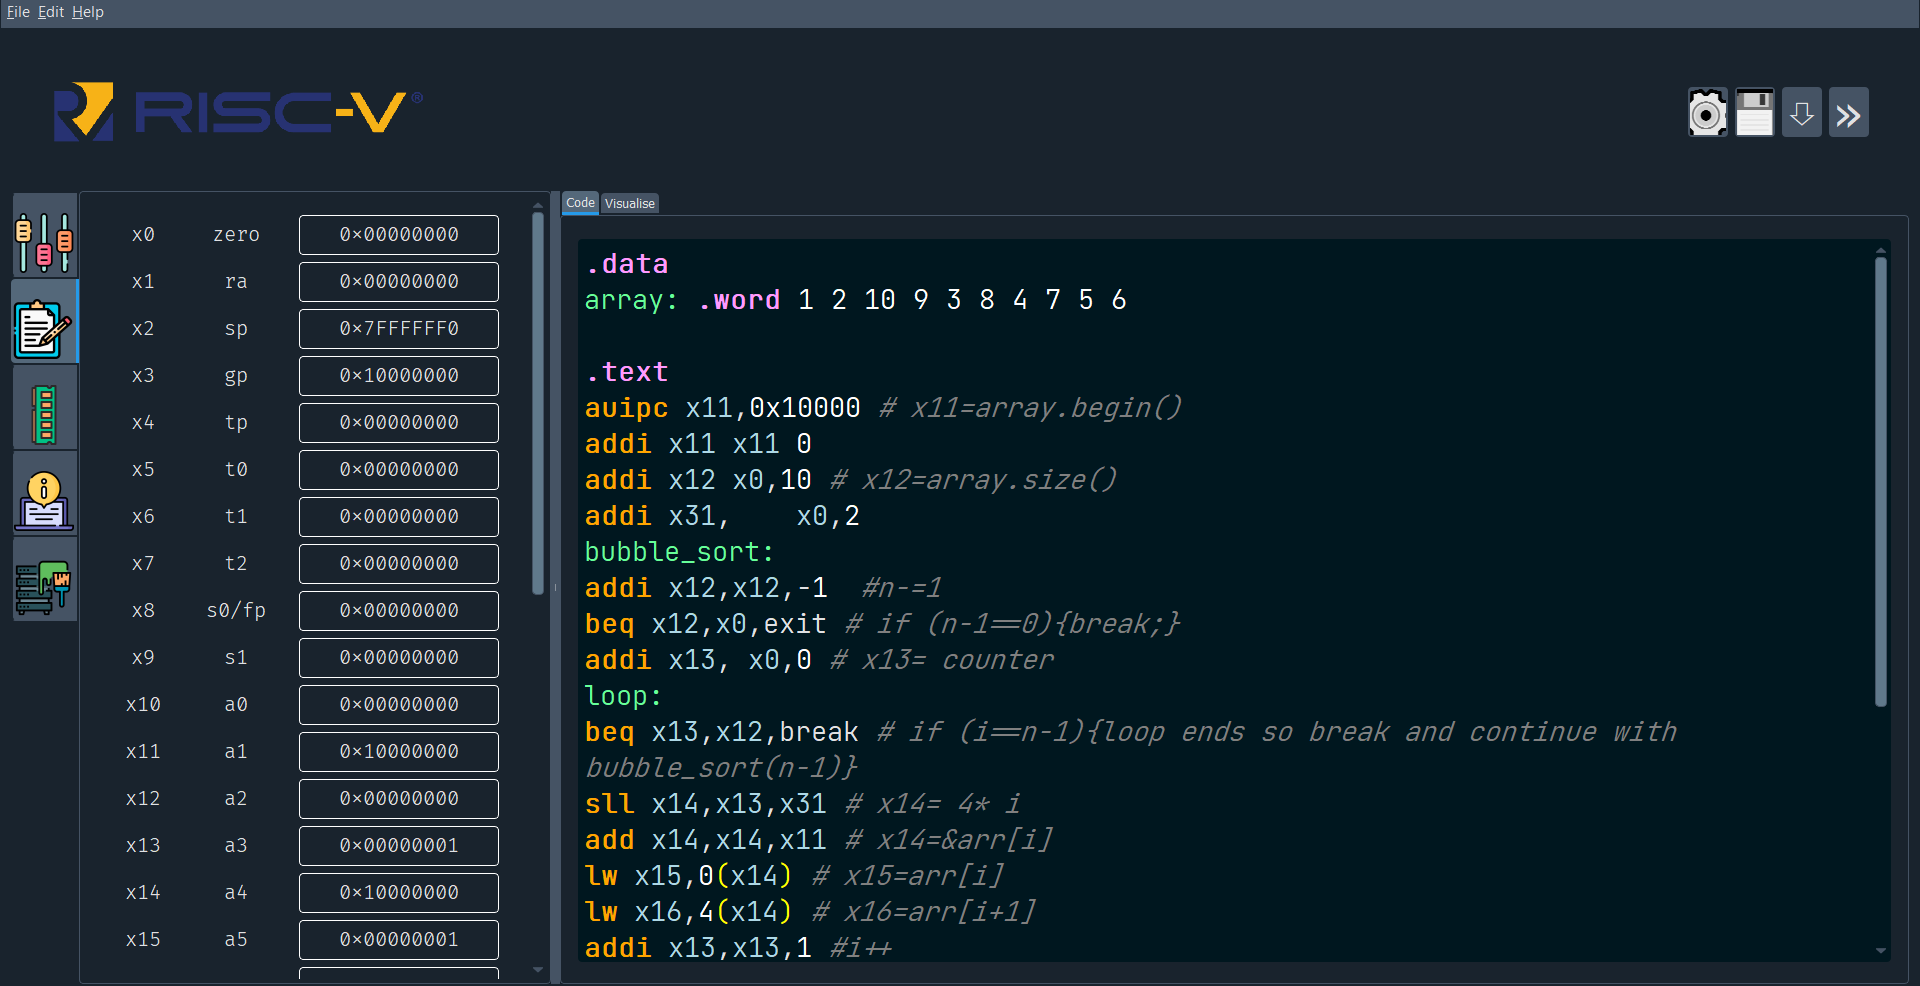
\includegraphics[width=1.0\textwidth]{RegistersPhase4.png}\vspace{2cm}
\end{centering}
We can see the values stored in all the Registers here. Values are stored in Hexadecimal format.\\
User can scroll down to observe the registers that are not immediately visible on the screen.





\newpage

\vspace{2cm}
\begin{centering}
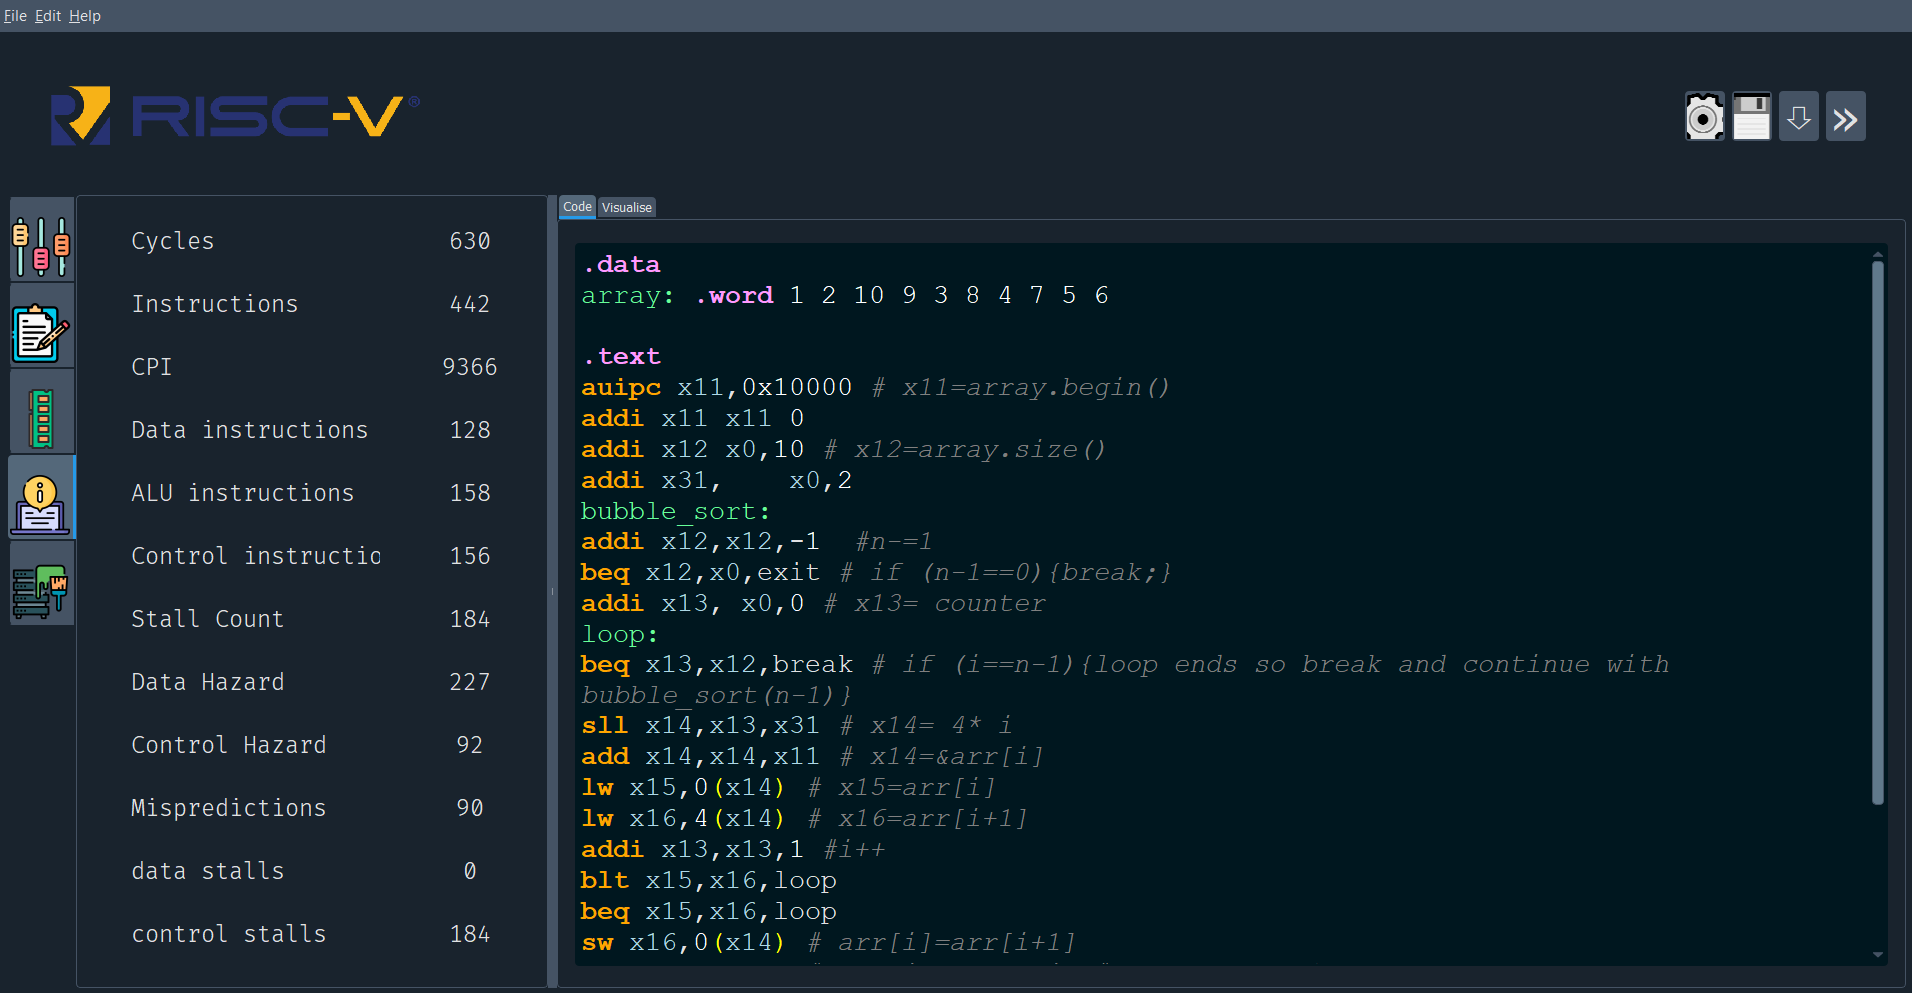
\includegraphics[width=1.0\textwidth]{Stats.png}\vspace{2cm}
\end{centering}
We can see the statistical details here\\



\newpage

\vspace{4cm}

\newpage

\begin{centering}
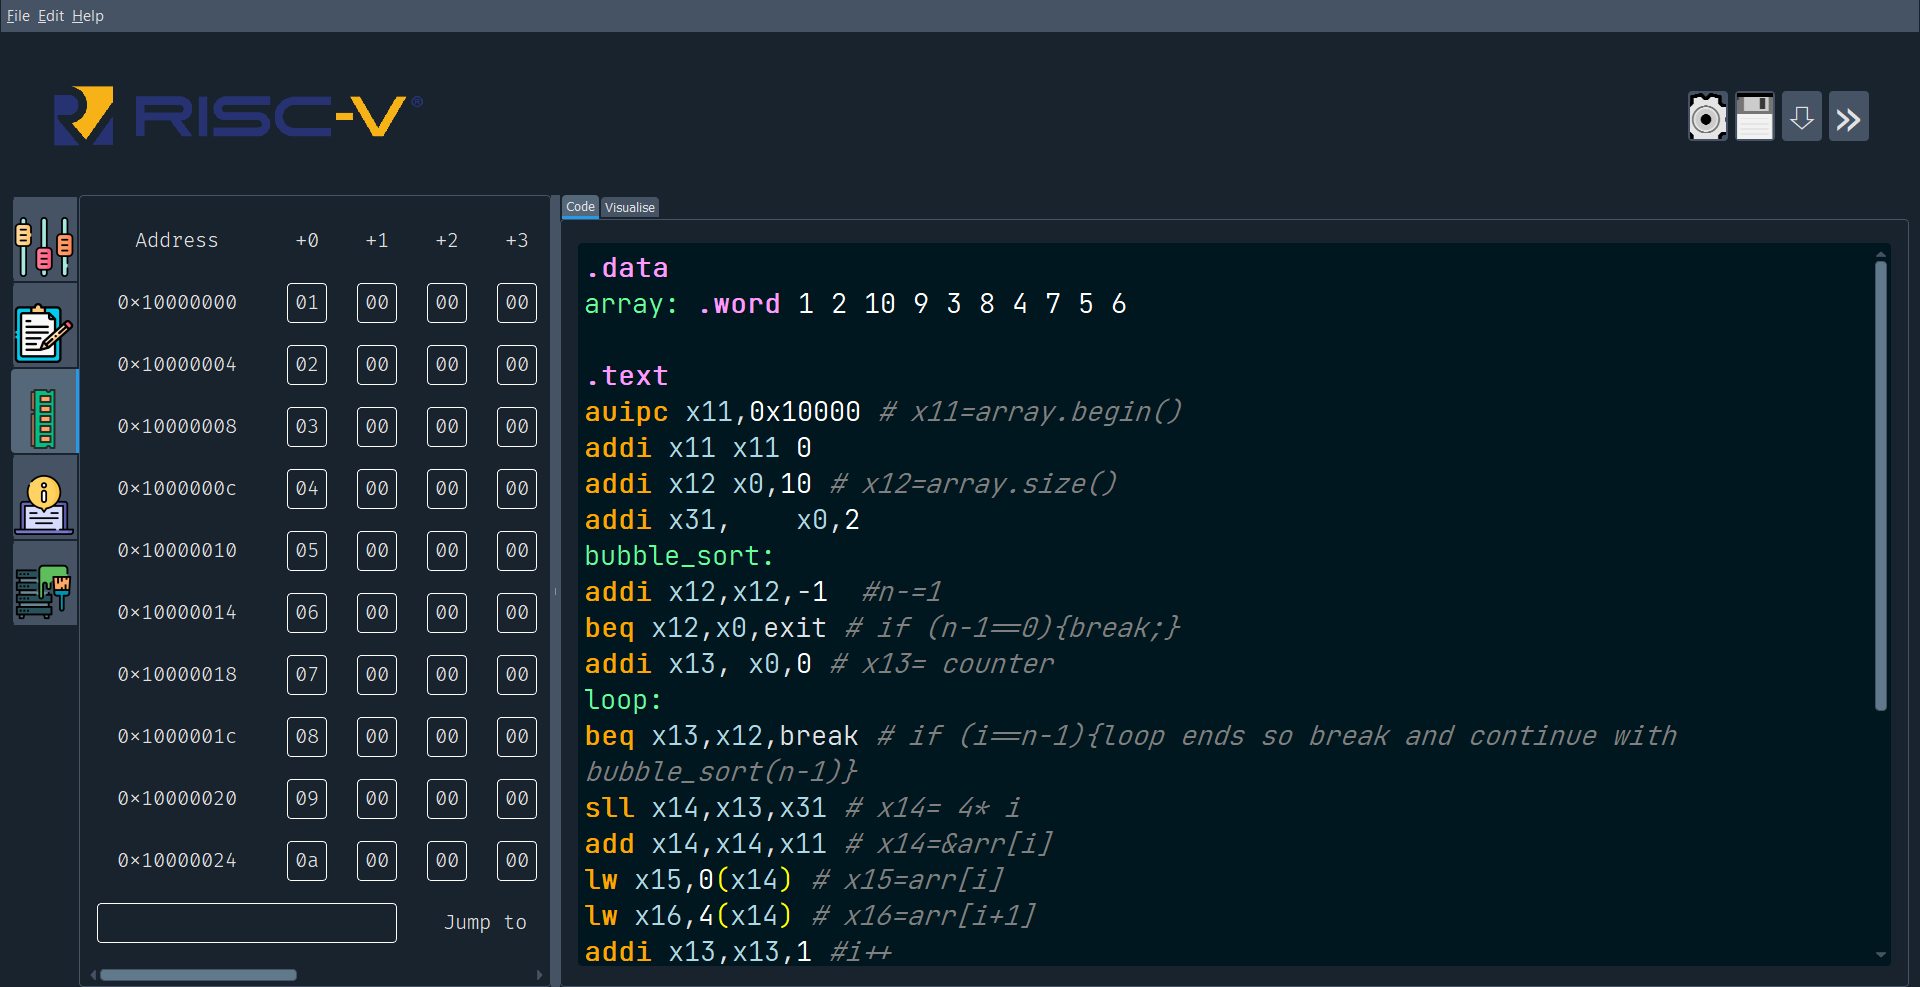
\includegraphics[width=1.0\textwidth]{MemoryPhase4.png}\vspace{2cm}
\end{centering}
\\
\LARGE
In the memory we can see the address and the value at each address. \\
For example if the address is 0x1000000C then the address of each of the right box are 0x1000000C , 0x1000000D, 0x1000000E and 0x1000000F.\\
Here we can see the jump to register functionality, where we have stored a value in the register 0x10000500, and are jumping to it and seeing the value.\\
\unindent
For example to jump on the location 0x10000500 write `10000500' in the Jump to box which is in the bottom right in the memory tab.


\newpage
\def\checkmark{\tikz\fill[scale=0.4](0,.35) -- (.25,0) -- (1,.7) -- (.25,.15) -- cycle;}
\LARGE
\\
\unindent
We have shown memory, registers and statistical details of the program on the left tabs of the GUI while on the right part there is Code Editor.\\
The code in the non Machine Version supports highlighting.\\
In the Code Editor you can edit your code or copy paste your code and also save it.\\
First of all we will paste the code in the Editor on the left side and then save and compile the code by clicking the respective `save' button which is the first button on the top right and `compile' button. The code will get updated in \textsl{\textbf{main.mc}} file and then the code will be executed and a \checkmark\hspace{0.7mm} will appear. The memory and registers will be updated simultaneously.\\\\
\unindent
Other details are present in their respective tabs as described earlier.\\\\


\newpage
\begin{centering}
\begin{Huge}
\textsf{Summary of the details of the layout of the GUI}\\
\end{Huge}
\vspace{0.6cm}
\end{centering}


\begin{itemize}
    \item We can jump to the memory using the `Jump to' box on the bottom right corner in the memory section.
    \item All the registers can be seen in the register file by scrolling in the register file section.
    \item We can execute non GUI code by writing \textrightarrow   python main.py
    \item We can set knob k1 k2 etc by using -k1 -k2 in the non GUI version.
    \item Executing \textsl{\textbf{python main.py -g}} always generates a GUI window where you can code in the Editor.
    \item In GUI we can tick the Pipelined, forwarding etc to execute the code in pipelined and forwarding manner respectively.
    \item We can observe all the register values in the register tab, Memory data in the memory tab and the statistical details in the Statistical tab.
\end{itemize}

\end{document}



